\documentclass[12pt]{article}
\usepackage{tikz}
\usepackage{geometry}

\usetikzlibrary{mindmap}

\author{Alan}
%2019-01-01
\geometry{landscape, margin=1cm}

\begin{document}
\begin{center}
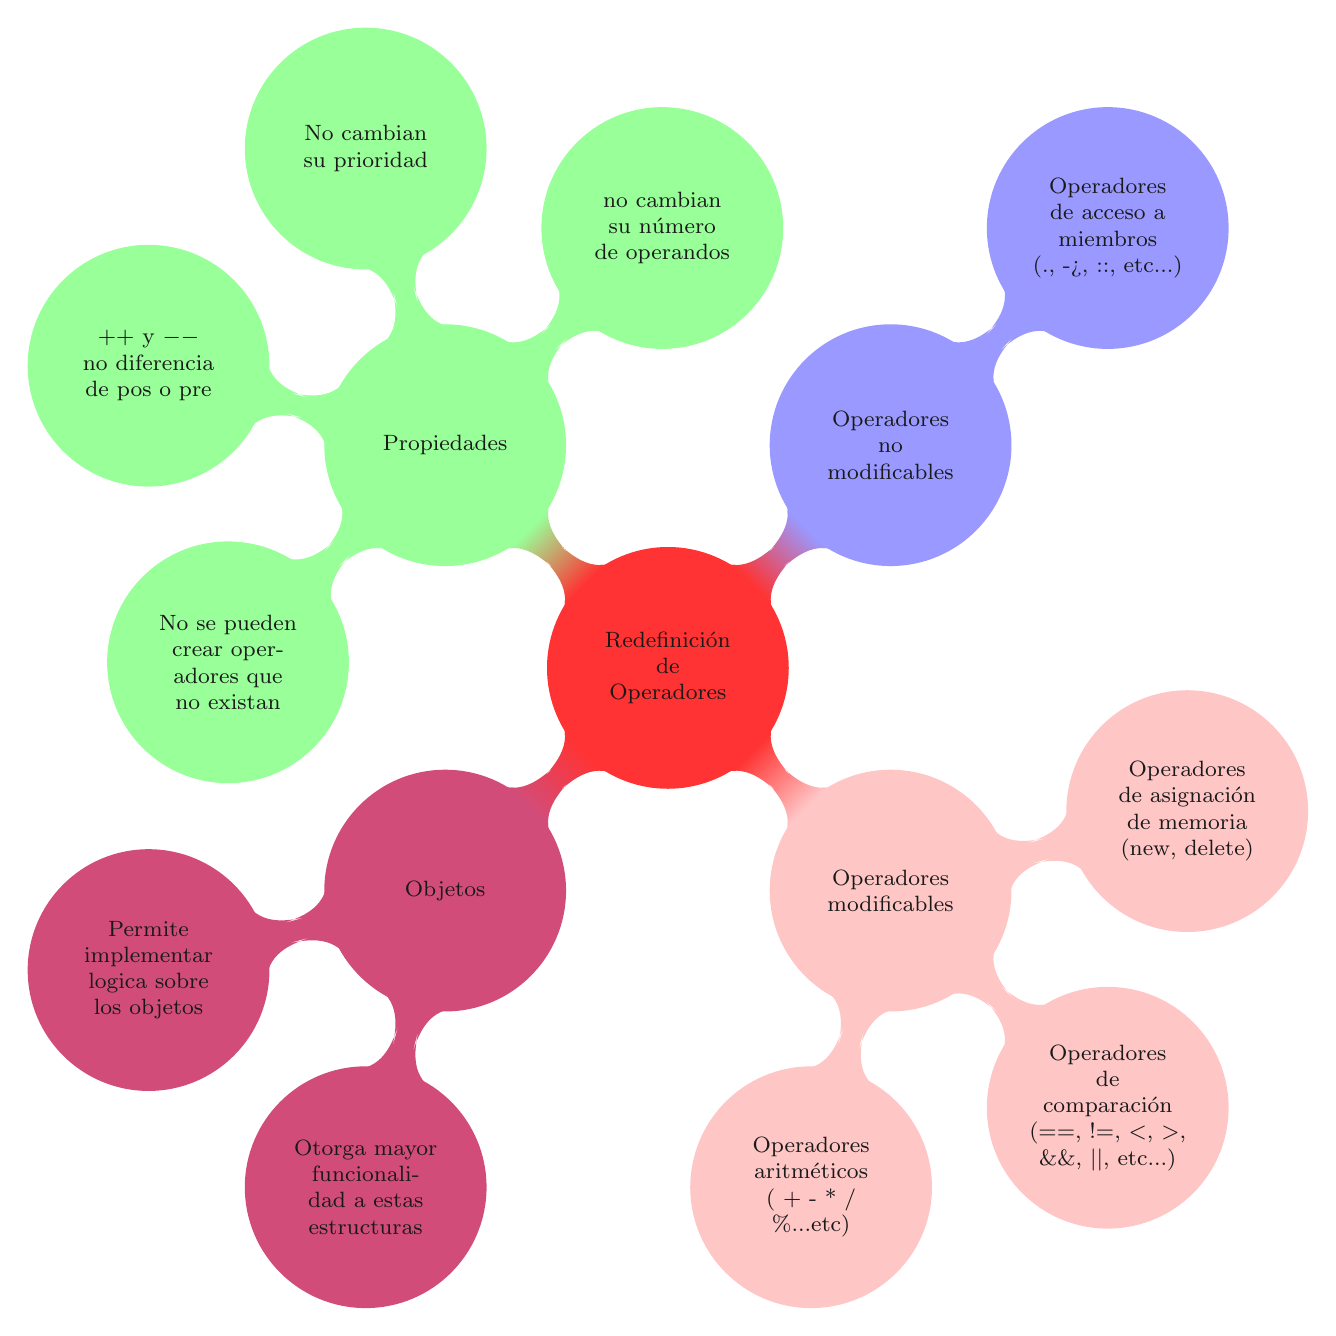
\begin{tikzpicture}[small mindmap, grow cyclic, every node/.style=concept, concept color=red!80, text=black!90, minimum size=3.0cm,
    level 1/.style={level distance=4.5cm,sibling angle=360/4},
    level 1/.style={level distance=4.0cm,sibling angle=360/4},
    level 2/.style={level distance=3.9cm,sibling angle=60},
    level 3/.style={level distance=3.5cm,sibling angle=60},
    ]
    \node{ Redefinición\\de\\Operadores }
    child[concept color=purple!70] { node { Objetos }
        child { node { Permite implementar logica sobre los objetos } }
        child { node { Otorga mayor funcionalidad a estas estructuras } }
    }
    child[concept color=pink!90] { node { Operadores modificables }
        child { node { Operadores\\aritméticos\\( + - * / \%...etc) } }
        child { node { Operadores\\de\\comparación\\(==, !=, $<$, $>$, \&\&, $\mid\mid$, etc...)  } }
        child { node { Operadores de asignación de memoria\\(new, delete) } }
    }
    child[concept color=blue!40] { node { Operadores\\no\\modificables }
        child { node { Operadores de acceso a miembros\\(., ->, ::, etc...) } }
    }
    child[concept color=green!40] { node { Propiedades }
        child { node { no cambian su número de operandos } }
        child { node { No cambian su prioridad } }
        child { node { ++ y $--$ no diferencia de pos o pre } }
        child { node { No se pueden crear operadores que no existan } }
    }
    ;
\end{tikzpicture}
\end{center}
\end{document}
